\section{User Requirements Definition}

La presente sezione descrive i requisiti utente e i casi d'uso del sistema \textbf{MyAma}, strutturati per classi di attori. Ciascun gruppo di casi d'uso è corredato dal relativo diagramma UML Use Case e dalle schede descrittive contenenti precondizioni, scenario principale, flussi alternativi ed eccezioni, postcondizioni e tracciabilità verso i requisiti di sistema.

% =========================================================================
% 3.1 UTENTE NON REGISTRATO / VISITATORE
% =========================================================================
\subsection{Use Case Utente Non Registrato / Visitatore}

\subsubsection{Diagramma dei Casi d'Uso: Utente Non Registrato}
\begin{figure}[H]
    \centering
    % \includegraphics[width=0.75\textwidth]{figure/uc_visitatore.png}
    \fbox{\parbox[c][5cm][c]{0.8\textwidth}{\centering \textsf{[ Inserire qui il Diagramma Use Case Utente Non Registrato esportato da Visual Paradigm ]}}}
    \caption{Use Case Diagram --- Utente Non Registrato / Visitatore}
    \label{fig:uc_visitatore}
\end{figure}

\subsubsection{Documentazione dei Casi d'Uso: Utente Non Registrato}

\usecasetable{UC-U01: Consultazione Informazioni e Tariffe}{
    Utente Non Registrato / Visitatore.
}{
    Il visitatore naviga sul portale MyAma per consultare le tipologie di rifiuti ingombranti trattati, le sedi territoriali attive e le relative tariffe.
}{
    Nessuna (accesso pubblico libero).
}{
    \begin{enumerate}[leftmargin=*]
        \item L'utente accede alla homepage di MyAma.
        \item Seleziona la sezione informativa sui servizi di smaltimento.
        \item Consulta le categorie di rifiuti ammissibili, le sedi disponibili e il tariffario comunale.
    \end{enumerate}
}{
    \begin{itemize}[leftmargin=*]
        \item \textbf{2a. Ricerca sede per CAP:} L'utente inserisce un CAP e il sistema mostra le isole ecologiche competenti più vicine.
    \end{itemize}
}{
    L'utente visualizza le informazioni richieste.
}{
    RF-01, RF-02.
}

\usecasetable{UC-U02: Registrazione al Sistema}{
    Utente Non Registrato / Visitatore.
}{
    Il visitatore compila il modulo di registrazione per creare un profilo Cittadino e poter prenotare i servizi di smaltimento.
}{
    L'utente non ha ancora un account attivo nel sistema.
}{
    \begin{enumerate}[leftmargin=*]
        \item L'utente seleziona l'opzione "Registrati".
        \item Inserisce i dati anagrafici e di contatto (Nome, Cognome, Codice Fiscale, Indirizzo di residenza, CAP, Email, Recapito Telefonico, Password).
        \item Prende visione e accetta l'informativa sul trattamento dei dati personali (Privacy).
        \item Invia la richiesta di registrazione.
        \item Il sistema valida i dati, registra l'account e invia un'email di conferma.
    \end{enumerate}
}{
    \begin{itemize}[leftmargin=*]
        \item \textbf{5a. Email o Codice Fiscale già registrato:} Il sistema segnala l'errore e propone il recupero credenziali.
        \item \textbf{5b. Formato dati non valido (es. CAP non valido o password debole):} Il sistema evidenzia i campi errati e richiede la correzione.
    \end{itemize}
}{
    Viene creato un nuovo profilo \textit{Cittadino Registrato} con credenziali attive.
}{
    RF-03, RNF-04.
}

% =========================================================================
% 3.2 CITTADINO REGISTRATO
% =========================================================================
\newpage
\subsection{Use Case Cittadino Registrato}

\subsubsection{Diagramma dei Casi d'Uso: Cittadino Registrato}
\begin{figure}[H]
    \centering
    % 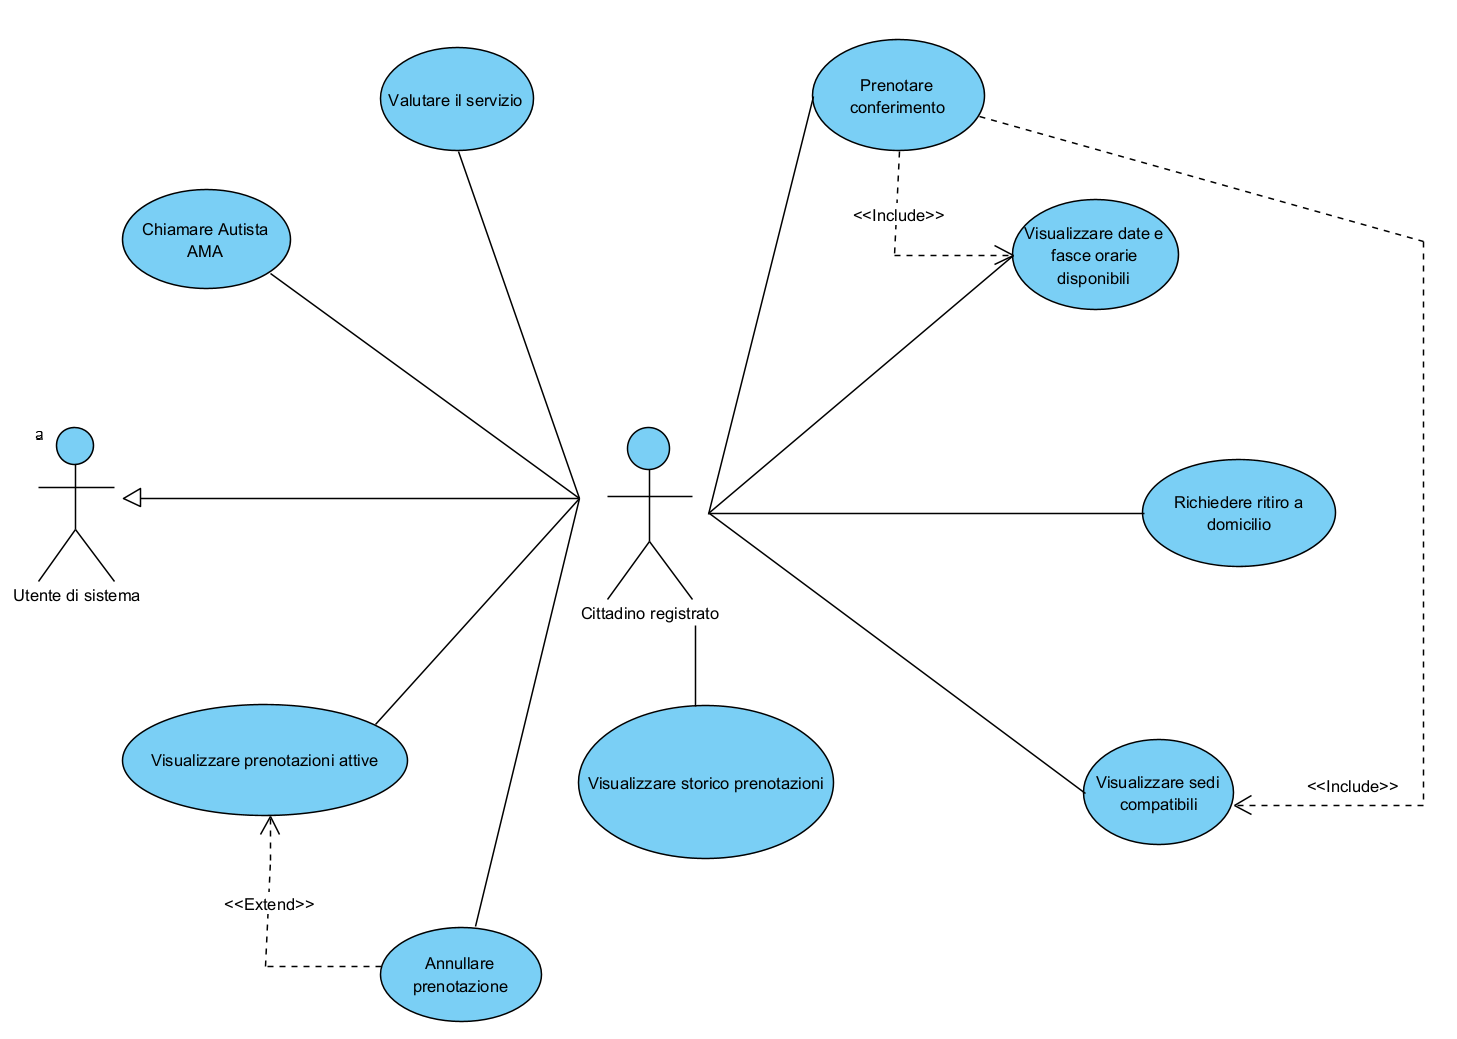
\includegraphics[width=0.85\textwidth]{figure/uc_cittadino.png}
    \fbox{\parbox[c][6.5cm][c]{0.8\textwidth}{\centering \textsf{[ Inserire qui il Diagramma Use Case Cittadino Registrato esportato da Visual Paradigm ]}}}
    \caption{Use Case Diagram --- Cittadino Registrato}
    \label{fig:uc_cittadino}
\end{figure}

\subsubsection{Documentazione dei Casi d'Uso: Cittadino Registrato}

\usecasetable{UC-C01: Prenotazione Ritiro a Domicilio}{
    Cittadino Registrato.
}{
    Il cittadino richiede il prelievo a domicilio di uno o più rifiuti ingombranti, specificando indirizzo, caratteristiche dei beni e selezionando uno slot orario disponibile.
}{
    Il cittadino ha effettuato l'accesso (login) al sistema.
}{
    \begin{enumerate}[leftmargin=*]
        \item Il cittadino seleziona la funzionalità "Prenota Ritiro a Domicilio".
        \item Inserisce la descrizione dei rifiuti (tipologia merceologica, quantità e dimensioni/peso stimato).
        \item Indica l'indirizzo di prelievo e il CAP di riferimento.
        \item Il sistema verifica che il CAP appartenga a una zona servita da AMA.
        \item Il sistema calcola e propone le date e fasce orarie disponibili in base al carico residuo dei veicoli e ai turni.
        \item Il cittadino seleziona lo slot orario desiderato.
        \item Il sistema mostra il riepilogo della prenotazione con l'eventuale tariffa calcolata.
        \item Il cittadino conferma la richiesta.
    \end{enumerate}
}{
    \begin{itemize}[leftmargin=*]
        \item \textbf{2a. Estensione Caricamento Foto Rifiuto (\texttt{<<extend>>}):} Il cittadino allega facoltativamente una o più fotografie del rifiuto per facilitare la stima volumetrica.
        \item \textbf{4a. CAP non servito:} Il sistema notifica la non copertura territoriale e suggerisce il conferimento diretto in sede.
        \item \textbf{5a. Nessuno slot compatibile nel periodo scelto:} Il sistema invita a consultare date successive.
    \end{itemize}
}{
    La prenotazione viene registrata con stato \textit{Confermata}, associata a un identificativo univoco e notificata al cittadino.
}{
    RF-04, RF-05, RF-06, RF-07, RD-01, RD-02.
}

\usecasetable{UC-C02: Prenotazione Conferimento in Sede}{
    Cittadino Registrato.
}{
    Il cittadino prenota un appuntamento per conferire direttamente rifiuti ingombranti o speciali presso un centro di raccolta AMA (isola ecologica).
}{
    Il cittadino ha effettuato l'accesso al sistema.
}{
    \begin{enumerate}[leftmargin=*]
        \item Il cittadino seleziona "Prenota Conferimento in Sede".
        \item Inserisce le tipologie di rifiuti da conferire e il proprio CAP.
        \item Il sistema visualizza le sedi/isole ecologiche abilitate alla ricezione di tali tipologie.
        \item Il cittadino sceglie la sede preferita e visualizza il calendario delle disponibilità.
        \item Seleziona data e fascia oraria.
        \item Conferma la prenotazione.
    \end{enumerate}
}{
    \begin{itemize}[leftmargin=*]
        \item \textbf{3a. Nessuna sede autorizzata per il rifiuto inserito:} Il sistema notifica i vincoli normativi sullo smaltimento speciale.
    \end{itemize}
}{
    La prenotazione viene registrata in stato \textit{Confermata} e viene generato un \textit{Pass di Conferimento} con codice univoco/QR code.
}{
    RF-08, RF-09, RF-10, RD-03.
}

\usecasetable{UC-C03: Consultazione Stato e Storico Prenotazioni}{
    Cittadino Registrato.
}{
    Il cittadino visualizza l'elenco di tutte le proprie richieste (attive e passate) e ne controlla lo stato di avanzamento.
}{
    Il cittadino è autenticato nel sistema.
}{
    \begin{enumerate}[leftmargin=*]
        \item Il cittadino accede alla sezione "Le mie prenotazioni".
        \item Il sistema recupera e mostra l'elenco delle prenotazioni con relativo stato (\textit{In attesa, Confermata, Completata, Annullata}).
        \item Il cittadino seleziona una specifica prenotazione per visualizzarne il dettaglio completo.
    \end{enumerate}
}{
    \begin{itemize}[leftmargin=*]
        \item \textbf{3a. Estensione Annullamento Prenotazione (\texttt{<<extend>>}):} Se la prenotazione è in stato \textit{Confermata} e mancano almeno 24 ore allo slot, il cittadino richiede l'annullamento; il sistema libera le risorse e imposta lo stato su \textit{Annullata}.
    \end{itemize}
}{
    Il cittadino ottiene il riepilogo aggiornato delle proprie richieste.
}{
    RF-11, RF-12, RD-04.
}

\usecasetable{UC-C04: Valutazione del Servizio}{
    Cittadino Registrato.
}{
    Il cittadino esprime una valutazione qualitativa su un servizio di smaltimento completato con successo.
}{
    La prenotazione di riferimento si trova in stato \textit{Completata}.
}{
    \begin{enumerate}[leftmargin=*]
        \item Il cittadino seleziona una prenotazione completata dal proprio storico.
        \item Seleziona l'opzione "Lascia una valutazione".
        \item Assegna un punteggio da 1 a 5 stelle e inserisce un commento testuale facoltativo.
        \item Invia il feedback.
    \end{enumerate}
}{
    \begin{itemize}[leftmargin=*]
        \item \textbf{4a. Valutazione già rilasciata:} Il sistema visualizza la valutazione precedentemente inserita in sola lettura.
    \end{itemize}
}{
    Il feedback viene registrato e associato alla prenotazione e alle statistiche di servizio.
}{
    RF-13.
}

% =========================================================================
% 3.3 AUTISTA AMA
% =========================================================================
\newpage
\subsection{Use Case Autista AMA}

\subsubsection{Diagramma dei Casi d'Uso: Autista AMA}
\begin{figure}[H]
    \centering
    % 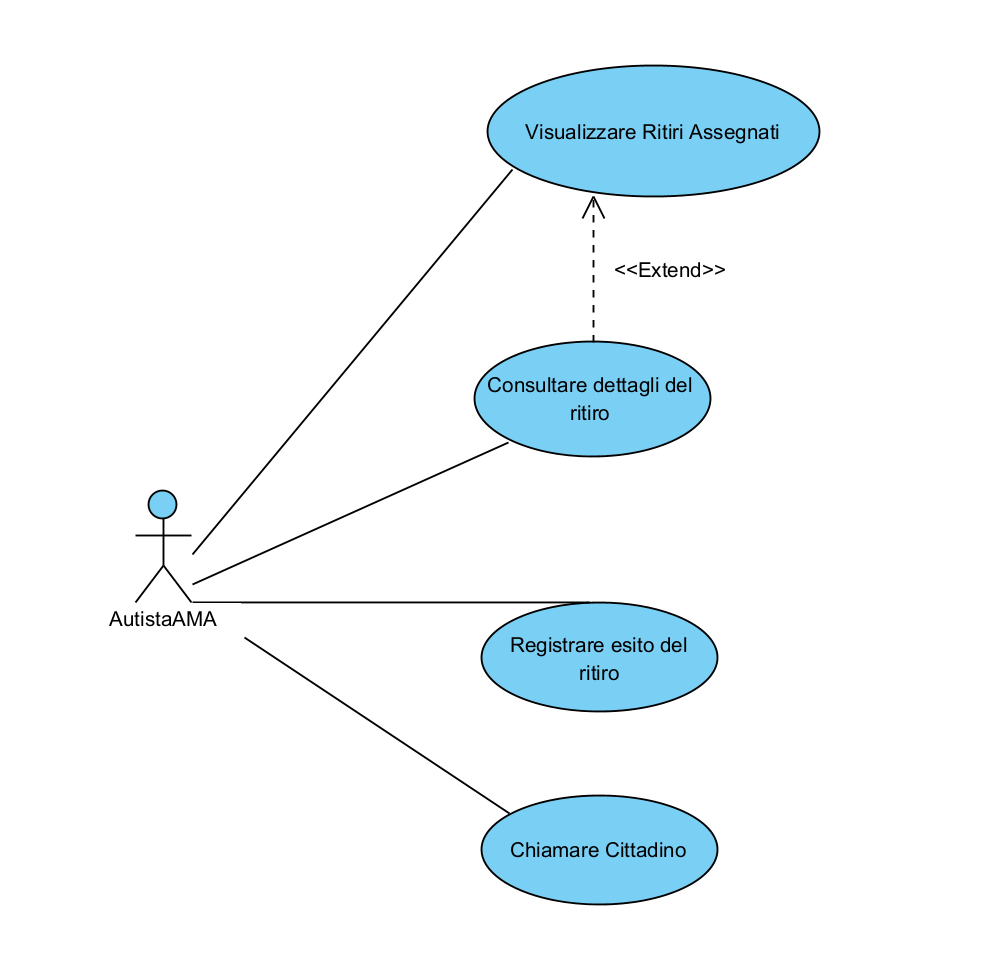
\includegraphics[width=0.8\textwidth]{figure/uc_autista.png}
    \fbox{\parbox[c][5.5cm][c]{0.8\textwidth}{\centering \textsf{[ Inserire qui il Diagramma Use Case Autista esportato da Visual Paradigm ]}}}
    \caption{Use Case Diagram --- Autista AMA}
    \label{fig:uc_autista}
\end{figure}

\subsubsection{Documentazione dei Casi d'Uso: Autista AMA}

\usecasetable{UC-A01: Consultazione Itinerario e Ritiri Assegnati}{
    Autista AMA.
}{
    L'autista consulta la lista ordinata dei ritiri a domicilio assegnati per il proprio turno, con dettagli su percorsi, orari, contatto del cittadino e carico.
}{
    L'autista ha effettuato l'accesso con profilo aziendale AMA.
}{
    \begin{enumerate}[leftmargin=*]
        \item L'autista accede all'applicazione MyAma Operatori.
        \item Il sistema carica l'itinerario giornaliero associato all'autista e al veicolo.
        \item L'autista visualizza la lista dei punti di ritiro e seleziona una scheda per visualizzare i dettagli (indirizzo, tipo di rifiuto, peso stimato, recapito).
    \end{enumerate}
}{
    \begin{itemize}[leftmargin=*]
        \item \textbf{2a. Nessun ritiro in programma:} Il sistema segnala l'assenza di assegnazioni per il turno selezionato.
    \end{itemize}
}{
    L'autista ottiene tutte le informazioni operative per svolgere il giro di raccolta.
}{
    RF-14, RF-15.
}

\usecasetable{UC-A02: Registrazione Esito Ritiro}{
    Autista AMA.
}{
    Al termine dell'intervento presso il domicilio del cittadino, l'autista formalizza il completamento del ritiro o l'eventuale mancata esecuzione.
}{
    L'autista ha raggiunto l'indirizzo della prenotazione in carico.
}{
    \begin{enumerate}[leftmargin=*]
        \item L'autista seleziona la prenotazione corrispondente.
        \item Seleziona l'esito: \textit{Completato con successo}.
        \item Inserisce eventuali annotazioni sul volume effettivo caricato.
        \item Conferma la registrazione dell'esito.
    \end{enumerate}
}{
    \begin{itemize}[leftmargin=*]
        \item \textbf{2a. Cittadino assente / Rifiuto non conforme:} L'autista registra l'esito \textit{Non Eseguito} o \textit{Rifiutato} indicando la motivazione formale (es. assenza al citofono, materiale vietato).
    \end{itemize}
}{
    Lo stato della prenotazione viene aggiornato a \textit{Completata} o \textit{Non Eseguita}, e il cittadino riceve una notifica automatica.
}{
    RF-16, RF-17.
}

\usecasetable{UC-A03: Contatto Cittadino}{
    Autista AMA.
}{
    L'autista invia un sollecito o contatta telefonicamente il cittadino in prossimità dell'arrivo all'indirizzo o in caso di difficoltà di accesso.
}{
    La prenotazione è attiva ed è in corso il turno di ritiro.
}{
    \begin{enumerate}[leftmargin=*]
        \item L'autista visualizza la scheda del ritiro corrente.
        \item Seleziona "Chiama Cittadino" o "Invia Notifica di Arrivo".
        \item Il sistema apre il canale di comunicazione/invia notifica push/SMS.
    \end{enumerate}
}{
    \begin{itemize}[leftmargin=*]
        \item \textbf{3a. Recapito non raggiungibile:} L'autista procede alla registrazione di mancato contatto nelle note.
    \end{itemize}
}{
    Il cittadino viene allertato dell'arrivo imminente dell'autista.
}{
    RF-18.
}

% =========================================================================
% 3.4 OPERATORE DI SEDE AMA
% =========================================================================
\newpage
\subsection{Use Case Operatore di Sede AMA}

\subsubsection{Diagramma dei Casi d'Uso: Operatore di Sede}
\begin{figure}[H]
    \centering
    % \includegraphics[width=0.8\textwidth]{figure/uc_operatore.png}
    \fbox{\parbox[c][5.5cm][c]{0.8\textwidth}{\centering \textsf{[ Inserire qui il Diagramma Use Case Operatore di Sede esportato da Visual Paradigm ]}}}
    \caption{Use Case Diagram --- Operatore di Sede AMA}
    \label{fig:uc_operatore}
\end{figure}

\subsubsection{Documentazione dei Casi d'Uso: Operatore di Sede}

\usecasetable{UC-O01: Consultazione Prenotazioni di Sede}{
    Operatore di Sede AMA.
}{
    L'operatore consulta l'elenco degli accessi e conferimenti programmati presso la propria isola ecologica per la giornata lavorativa.
}{
    L'operatore è autenticato e associato alla sede di servizio.
}{
    \begin{enumerate}[leftmargin=*]
        \item L'operatore accede al pannello operativo di sede.
        \item Visualizza la timeline degli slot di conferimento ordinati per orario.
        \item Consulta il volume atteso e le tipologie di rifiuti previste.
    \end{enumerate}
}{
    \begin{itemize}[leftmargin=*]
        \item \textbf{2a. Filtro per codice o nominativo:} L'operatore ricerca una specifica prenotazione inserendo il codice pass.
    \end{itemize}
}{
    L'operatore visualizza il quadro delle accettazioni previste.
}{
    RF-19.
}

\usecasetable{UC-O02: Convalida e Registrazione Conferimento al Varco}{
    Operatore di Sede AMA.
}{
    All'arrivo del cittadino al varco del centro di raccolta, l'operatore verifica il pass, controlla visivamente la conformità dei rifiuti e convalida lo scarico.
}{
    Il cittadino è presente presso l'isola ecologica con prenotazione attiva.
}{
    \begin{enumerate}[leftmargin=*]
        \item L'operatore scansiona il QR code del pass di conferimento (o inserisce il codice alfanumerico).
        \item Il sistema convalida il pass e mostra i dati del conferimento.
        \item L'operatore ispeziona il carico accertando la conformità con la tipologia dichiarata.
        \item Registra l'avvenuto scarico con esito \textit{Completato}.
    \end{enumerate}
}{
    \begin{itemize}[leftmargin=*]
        \item \textbf{2a. Pass non valido o già utilizzato:} Il sistema segnala l'anomalia all'operatore.
        \item \textbf{3a. Presenza di rifiuti non conformi o pericolosi non ammessi:} L'operatore respinge parzialmente o totalmente il conferimento e registra la non conformità.
    \end{itemize}
}{
    La prenotazione viene archiviata con stato \textit{Completata} o \textit{Respinta}.
}{
    RF-20, RF-21, RD-03.
}

% =========================================================================
% 3.5 AMMINISTRATORE DI SEDE AMA
% =========================================================================
\newpage
\subsection{Use Case Amministratore di Sede AMA}

\subsubsection{Diagramma dei Casi d'Uso: Amministratore di Sede}
\begin{figure}[H]
    \centering
    % 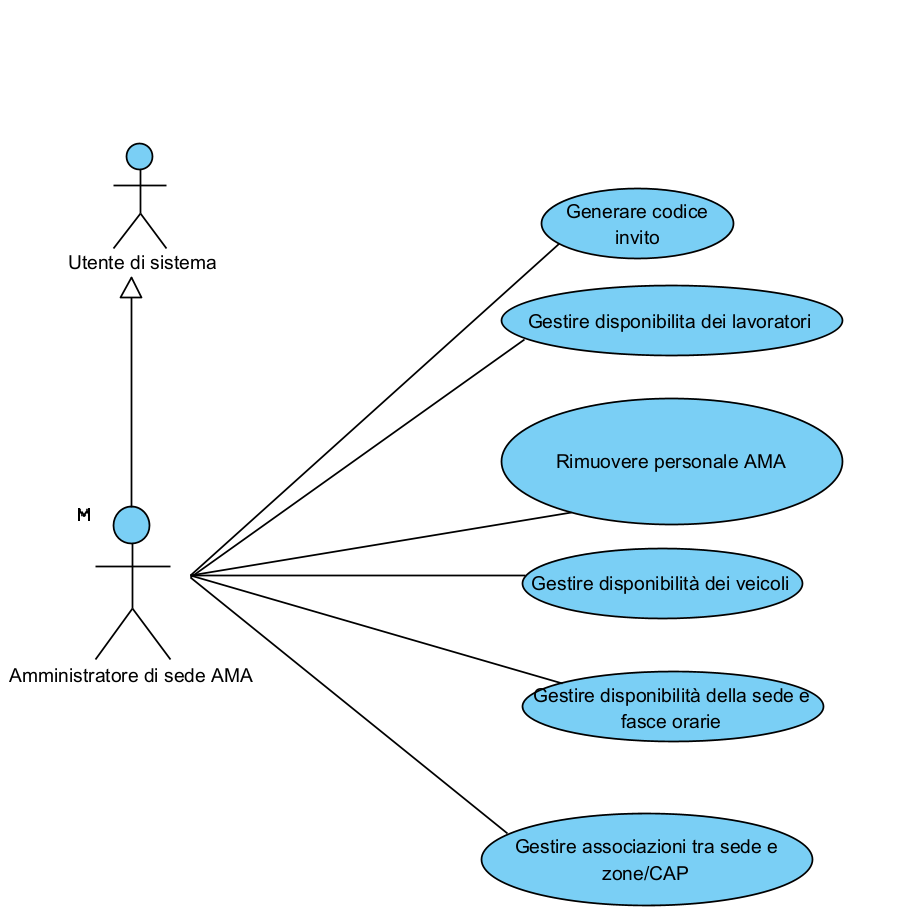
\includegraphics[width=0.8\textwidth]{figure/uc_amministratore_sede.png}
    \fbox{\parbox[c][5.5cm][c]{0.8\textwidth}{\centering \textsf{[ Inserire qui il Diagramma Use Case Amministratore di Sede esportato da Visual Paradigm ]}}}
    \caption{Use Case Diagram --- Amministratore di Sede AMA}
    \label{fig:uc_amm_sede}
\end{figure}

\subsubsection{Documentazione dei Casi d'Uso: Amministratore di Sede}

\usecasetable{UC-S01: Gestione Personale e Turni Sede}{
    Amministratore di Sede AMA.
}{
    L'amministratore di sede gestisce l'anagrafica degli autisti e degli operatori assegnati alla propria struttura, configurando i turni settimanali.
}{
    L'amministratore ha effettuato l'accesso con profilo di sede abilitato.
}{
    \begin{enumerate}[leftmargin=*]
        \item L'amministratore accede al pannello "Gestione Personale".
        \item Visualizza i lavoratori in organico con relative mansioni e disponibilità.
        \item Definisce o aggiorna la pianificazione dei turni per la settimana/mese.
        \item Salva la configurazione operativa.
    \end{enumerate}
}{
    \begin{itemize}[leftmargin=*]
        \item \textbf{3a. Sovrapposizione di turni o carenza organico minimo:} Il sistema evidenzia un alert di pianificazione.
    \end{itemize}
}{
    I turni del personale risultano configurati e disponibili per l'allocazione delle prenotazioni.
}{
    RF-22, RF-23.
}

\usecasetable{UC-S02: Gestione Veicoli e Disponibilità Mezzi}{
    Amministratore di Sede AMA.
}{
    L'amministratore censisce i veicoli operativi della sede, impostando portata massima (kg) e volume utile ($m^3$) per la flotta di ritiro.
}{
    L'amministratore è autenticato nel pannello di sede.
}{
    \begin{enumerate}[leftmargin=*]
        \item Accede alla sezione "Parco Veicoli".
        \item Visualizza i mezzi disponibili e ne aggiorna lo stato operativo (\textit{Disponibile, In manutenzione, Fuori servizio}).
        \item Associa i veicoli disponibili ai turni di ritiro programmati.
    \end{enumerate}
}{
    \begin{itemize}[leftmargin=*]
        \item \textbf{2a. Mezzo impostato in manutenzione:} Il sistema impedisce nuove assegnazioni su quel mezzo fino al ripristino.
    \end{itemize}
}{
    Le disponibilità dei mezzi vengono aggiornate per il calcolo degli slot ai cittadini.
}{
    RF-24, RD-01.
}

\usecasetable{UC-S03: Configurazione Sede e Associazione Zone/CAP}{
    Amministratore di Sede AMA.
}{
    L'amministratore definisce gli orari di apertura del centro di raccolta e aggiorna i CAP serviti per i ritiri a domicilio.
}{
    L'amministratore è autenticato.
}{
    \begin{enumerate}[leftmargin=*]
        \item Accede alla sezione "Configurazione Territoriale e Orari".
        \item Definisce le fasce orarie di apertura per il conferimento dei cittadini.
        \item Associa o modifica i CAP comunali di competenza della propria sede.
        \item Conferma le modifiche.
    \end{enumerate}
}{
    \begin{itemize}[leftmargin=*]
        \item \textbf{3a. CAP già associato a sede prioritaria:} Il sistema notifica la ripartizione del bacino d'utenza.
    \end{itemize}
}{
    I parametri territoriali della sede risultano aggiornati nel motore di verifica CAP.
}{
    RF-25, RD-02.
}

% =========================================================================
% 3.6 AMMINISTRATORE GENERALE AMA
% =========================================================================
\newpage
\subsection{Use Case Amministratore Generale AMA}

\subsubsection{Diagramma dei Casi d'Uso: Amministratore Generale}
\begin{figure}[H]
    \centering
    % 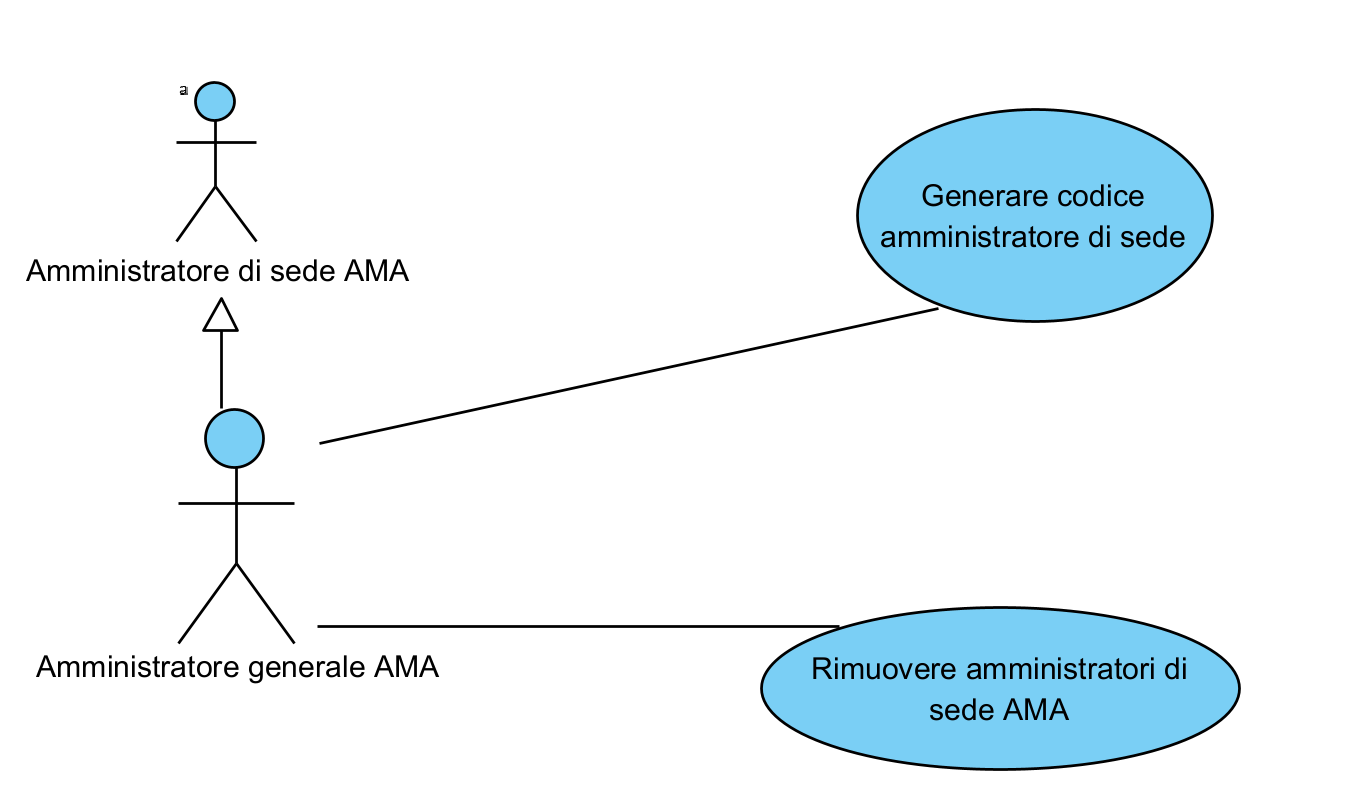
\includegraphics[width=0.8\textwidth]{figure/uc_amministratore_generale.png}
    \fbox{\parbox[c][5.5cm][c]{0.8\textwidth}{\centering \textsf{[ Inserire qui il Diagramma Use Case Amministratore Generale esportato da Visual Paradigm ]}}}
    \caption{Use Case Diagram --- Amministratore Generale AMA}
    \label{fig:uc_amm_generale}
\end{figure}

\subsubsection{Documentazione dei Casi d'Uso: Amministratore Generale}

\usecasetable{UC-G01: Gestione Account Amministratori di Sede}{
    Amministratore Generale AMA.
}{
    La direzione aziendale gestisce gli account dei responsabili di sede, abilitando o revocando le credenziali di accesso al pannello gestionale.
}{
    L'utente è autenticato con privilegi di Amministratore Generale.
}{
    \begin{enumerate}[leftmargin=*]
        \item L'amministratore generale accede al modulo "Amministrazione Sedi".
        \item Crea un nuovo profilo Amministratore di Sede associandolo alla struttura territoriale di competenza.
        \item Invia le credenziali di primo accesso al responsabile nominato.
    \end{enumerate}
}{
    \begin{itemize}[leftmargin=*]
        \item \textbf{2a. Revoca o disattivazione incarico:} L'amministratore generale disabilita l'accesso all'account di sede.
    \end{itemize}
}{
    L'anagrafica dei responsabili di sede risulta aggiornata.
}{
    RF-26.
}

\usecasetable{UC-G02: Consultazione Reportistica e Statistiche Globali}{
    Amministratore Generale AMA.
}{
    La direzione analizza indicatori di performance e report aggregati sui flussi di rifiuti smaltiti in tutta la città.
}{
    L'utente è autenticato come Amministratore Generale.
}{
    \begin{enumerate}[leftmargin=*]
        \item Accede alla dashboard "Reportistica \& Analytics".
        \item Seleziona filtri temporali (settimana, mese, anno) e territoriali (distretti/CAP).
        \item Consulta grafici e tabelle su: volume totale rifiuti ritirati, percentuale di successo ritiri, tasso di saturazione centri di raccolta e valutazioni medie dei cittadini.
    \end{enumerate}
}{
    \begin{itemize}[leftmargin=*]
        \item \textbf{3a. Esportazione dati:} L'amministratore esporta i dati in formato standard (PDF/CSV) per relazioni dirigenziali.
    \end{itemize}
}{
    L'amministratore ottiene la vista analitica complessiva per il monitoraggio aziendale.
}{
    RF-27.
}
